%% LyX 2.1.4 created this file.  For more info, see http://www.lyx.org/.
%% Do not edit unless you really know what you are doing.
\documentclass[oneside,english]{amsart}
\usepackage[T1]{fontenc}
\usepackage[latin9]{inputenc}
\usepackage[landscape]{geometry}
\geometry{verbose,tmargin=0.5in,bmargin=0.5in,lmargin=1.25in,rmargin=1.25in}
\setlength{\parskip}{\smallskipamount}
\setlength{\parindent}{0pt}
\usepackage{float}
\usepackage{amsthm}
\usepackage{amssymb}

\makeatletter

%%%%%%%%%%%%%%%%%%%%%%%%%%%%%% LyX specific LaTeX commands.
%% Because html converters don't know tabularnewline
\providecommand{\tabularnewline}{\\}

%%%%%%%%%%%%%%%%%%%%%%%%%%%%%% Textclass specific LaTeX commands.
\numberwithin{equation}{section}
\numberwithin{figure}{section}
\usepackage{enumitem}		% customizable list environments
\newlength{\lyxlabelwidth}      % auxiliary length 

%%%%%%%%%%%%%%%%%%%%%%%%%%%%%% User specified LaTeX commands.
\usepackage{hyperref}
\usepackage[usenames,dvipsnames,table]{xcolor} %adds additional color options
\hypersetup{colorlinks=true, urlcolor=black,linkcolor=black}

\usepackage{fancyhdr}
\usepackage{lastpage}
\pagestyle{fancy}
\usepackage{enumitem}
\usepackage{ifthen}
%sets math fonts to be more readable
\everymath=\expandafter{\the\everymath\displaystyle}
\DeclareMathSizes{10}{10}{10}{10}
\usepackage{multicol}

\usepackage{tikz}
\usepackage{tkz-euclide} %%angle marks and such
% removed: usetkzobj is obsolete in tkz-euclide 3+
\usetikzlibrary{plotmarks}
\usepackage{pgfplots}
\pgfplotsset{compat=newest}
\usepackage{amssymb}

\usepackage{calc}
%%\usepackage[nomessages]{fp} clashes with tkz-euclide?

%\usepackage{advdate}    % Advancing/saving dates
\usepackage{datetime}   % Dates formatting
%\usepackage{datenumber} % Counters for dates
\newdateformat{MD}{\monthname[\THEMONTH] \ordinal{DAY}}

\def\formatdateny{\csname noyear\languagename\expandafter\endcsname\formatdate}
\def\noyearenglish#1, \the\@year{#1}
\let\noyearamerican\noyearenglish
\let\noyearbritish\noyearenglish

\usepackage{fancybox} %%ovalbox and fancy box settings

\usepackage[outline]{contour}  %allows text halos
\usepackage{colortbl}


\usepackage[super]{nth} %easy 1st, 2nd, etc

\usepackage{forest} %%for tree diagram
\usepackage{caption}%%allows turing off numbers on fig
\usepackage{fontawesome} %%for \faBirthdayCake
\usepackage{pgf-pie}

\makeatother

\usepackage{babel}
\begin{document}
\renewcommand{\author}{WGU Math Center}

\newcommand{\classNum}{}

\newcommand{\classSec}{}

\newcommand{\nameType}{}

\newcommand{\examType}{Praxis Core Practice: Math (5732)}

\renewcommand{\date}{\today}

%%First page's header%%%%%%%%%%%%%%%%%%%%%%
\fancypagestyle{firststyle} %%header settings for first pagr
{
	\fancyhead[L]{\author}
	\fancyhead[C]{\textbf{\examType}}

head{}
	\lfoot{\date}

	\setlength{\headsep}{30pt}
}
%%%%%%%%%%%%%%%%%%%%%%%%%%%%%%%%%%%%%%%%%%

%%Next page's header%%%%%%%%%%%%%%%%%%%%%%%
%\setlist{nolistsep}
\lhead{\author} 
\chead{\textbf{\examType}} 
\cfoot{\thepage{}~of~\pageref{LastPage}} 

head{}

\setlength{\headsep}{30pt}
%%%%%%%%%%%%%%%%%%%%%%%%%%%%%%%%%%%%%%%%%%%%%Various settings; see the preamble for other settings%%%%%
%%\setenumerate[0]{leftmargin=12pt,itemindent=0pt,labelwidth=0pt}
%\setlist[2]{noitemsep}
%\setlist{nosep}
\setlist{itemsep=8pt,topsep=12pt} %,parsep=0pt}
\setlength\multicolsep{3pt}
\setlength{\parindent}{0pt} %%no indent
\renewcommand{\labelenumi}{\textbf{\arabic{enumi}.}}
\renewcommand{\labelenumii}{\textbf{\alph{enumii}.}}
\thispagestyle{firststyle}

%%%%%%For problem type%%%%%%%%%%%%%%%%%%%%
%\newcommand{\clicking}{\textbf{clicking on}~}
\newcommand{\clicking}{\textbf{choosing}~}
%\newcommand{\click}{\textbf{~Click on~}}
\newcommand{\click}{\textbf{~Indicate all~}}

\newcommand{\questMulti}{\renewcommand\labelitemi{\myEllipse} \textbf{Answer the question below by }\clicking\textbf{the correct response.} \\ \\~}

\newcommand{\questMultiPic}{\renewcommand\labelitemi{\myEllipse} \textbf{Answer the question below by }\clicking\textbf{the correct response.}}

\newcommand{\questFill}{\textbf{Write your answer in the provided form.} \\ \\}

\newcommand{\questFillPic}{\textbf{Write your answer in the provided form.}}

\newcommand{\questInd}{\renewcommand\labelitemi{\myBox}  \textbf{Indicate all of your answers.} \\ \\}
   
%%%%%%%%%%%%%%%%%%%%%%%%%%%%%%%%%%%%%%%%%%
\newcommand{\xmax}{10}
\newcommand{\xmin}{-10}
\newcommand{\xstep}{0} %must be xmin+n
\newcommand{\ymax}{10}
\newcommand{\ymin}{-10}
\newcommand{\ystep}{0} %must be ymin+n

%%comments%%
\definecolor{readablegreen}{rgb}{0,0.4,0}

%%%macros%%%
\newcommand{\gWidth}{6cm}
\newcommand{\gHeight}{6cm}
\newcommand{\Scale}{1.0}
\newcommand{\textSize}{\normalsize}

%%%options%%
%\tiny \scriptsize \footnotesize \small \normalsize, \large, \Large, \LARGE, \huge, \Huge
\newcommand{\examTextSize}{\LARGE}
\examTextSize
\newcommand{\multi}{\cdot}
\newcommand{\xspace}{\hspace*{0pt}}
\newcommand{\yspace}{\vspace{0pt} \newpage} %1.4cm

%%%for bubbles and boxes%%%%%
\newcommand*{\ansEllipse}{ 	
	\begin{tikzpicture} 		
	\draw[black,thick, fill=readablegreen] (0,0) ellipse (.35cm and .185cm); 	
	\end{tikzpicture} 	
	} 

\newcommand*{\myEllipse}{
	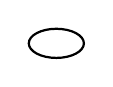
\begin{tikzpicture}
		\draw[thick] (0,0) ellipse (.35cm and .185cm);
	\end{tikzpicture}
	}

\newcommand*{\ansBox}{
	\begin{tikzpicture}
		\draw[thick,fill=readablegreen] (0,0) rectangle (.325,.325);
	\end{tikzpicture}
	}

\newcommand*{\myBox}{ 	
	
\begin{tikzpicture} 		
		\draw[thick] (0,0) rectangle (.325,.325);
	\end{tikzpicture}
	}

%%%%%Answers%%%%%%%%%%%%%%%%%%%%%%%%%%%%%%%%%%%%%%%%%%%%
%%%%%\quest micros set labelitemi for boxes or ovals%%%%
%%Turn answers off/on by uncommenting/commenting renewcommands%%%
\newcommand{\ansE}{\ansEllipse}
\newcommand{\ansB}{\ansBox}
\newcommand{\answer}[1]{\textbf{\textcolor{readablegreen}{#1}}} 
\renewcommand{\ansE}{\myEllipse}
\renewcommand{\ansB}{\myBox}
\renewcommand{\answer}[1]{\textbf{\textcolor{white}{#1}}}

%%%options%%
\renewcommand{\textSize}{\normalsize}
%\tiny \scriptsize \footnotesize \small \normalsize, \large, \Large, \LARGE, \huge, \Huge
\renewcommand{\examTextSize}{\LARGE}
\examTextSize
\renewcommand{\multi}{\cdot}
\renewcommand{\xspace}{\hspace*{0pt}}
\renewcommand{\yspace}{\vspace{0pt} \newpage} %1.4cm
\begin{enumerate}[resume]
\item \questMultiPic \renewcommand{\textSize}{\large}
\begin{figure}[H]
\begin{center}%%%%graph with grid and labels 
\renewcommand{\xmax}{12} 
\renewcommand{\xmin}{0} 
\renewcommand{\xstep}{0} %must be xmin+n 
\renewcommand{\ymax}{200} 
\renewcommand{\ymin}{0} 
\renewcommand{\ystep}{0} %must be ymin+n %%%%%%% 
\begin{tikzpicture}  
\begin{axis}[ 	
	height=7cm,  	
	width=6cm,  	
	axis lines=middle, 	
	ymax=\ymax, ymin=\ymin,	
	xmax=\xmax, xmin=\xmin,
	grid=both, 	
	xtick={0,2,4,...,20}, 	
	ytick={0,20,40,...,180}, 	
	%every axis x label/.append style={anchor=west},  	
	%every axis y label/.append style={anchor=south},	 	
	x label style={at={(axis description cs:0.5,-0.15)},anchor=north},
	y label style={at={(axis description cs:-0.25,0.5)},rotate=90,anchor=south}, 	
	xlabel={\textSize Number of Couples}, 	
	ylabel={\textSize Total Cost (in dollars)}, 	
	clip=false, %doesn't clip outside graph 	
	] 	
	\addplot[-latex,domain=\xmin:\xmax-.25,samples=100,draw=black]{15*x+10} [yshift=5pt] node[pos=0.5,above] {$$}; 
\end{axis} 
\end{tikzpicture}\end{center}
\end{figure}
 \noindent The graph above shows the relationship between the cost
of a luncheon and the number of people attending the luncheon. According
to the graph, what is the cost per couple? \\


\begin{itemize}
\item $\$14.00$
\item [\ansE]$\$15.00$
\item $\$17.50$
\item $\$20.00$
\item $\$30.00$\yspace \vfill
\end{itemize}
\item \questMulti A fair coin is labeled \textquotedbl{}H\textquotedbl{}
on one side and \textquotedbl{}T\textquotedbl{} on the other side.
Stephen flips the coin 6 times and the result is H, H, T, H, H, H.
What is the probability that the result will be a T on his seventh
flip?

\begin{itemize}
\item $\frac{1}{7}$
\item $\frac{1}{6}$
\item $\frac{1}{3}$
\item [\ansE]$\frac{1}{2}$
\item $\frac{5}{6}$\yspace \vfill
\end{itemize}
\item \questMulti Which of the following expressions is equivalent to the
expression $15-6x$ for all values of $x$?

\begin{itemize}
\item $5+3(5-2x)$
\item $18-(3-6x)$
\item [\ansE]$19-2(2+3x)$
\item $3(2-2x)+10$
\item $2(5-6x)+25$\yspace \vfill
\end{itemize}
\item \questMulti Jim observed that the more time his students spent studying
for the Praxis the higher their scores were. Which of the following
graphs best describes the relationship Jim observed between time students
spent studying and their test scores? \renewcommand{\gWidth}{5cm}
\renewcommand{\gHeight}{4.375cm}
\renewcommand{\xmax}{10}
\renewcommand{\xmin}{0}
\renewcommand{\xstep}{0} %must be xmin+n
\renewcommand{\ymax}{10}
\renewcommand{\ymin}{0}
\renewcommand{\ystep}{0} %must be ymin+n
\renewcommand{\textSize}{\normalsize}


\begin{multicols}{2}
\begin{itemize}
\item %
\begin{minipage}[c][1\totalheight][t]{1\columnwidth}%
%%%%%%%
\begin{tikzpicture} 
\begin{axis}[
	height=\gHeight, 
	width=\gWidth, 
	axis lines=middle,
	grid=none,
	ticks=none,
	axis line style={-latex}, 
	xmin=\xmin,xmax=\xmax, 
	ymin=\ymin,ymax=\ymax,
	no markers, 
	x label style={at={(axis description cs:0.5,-0.0)},anchor=north},     
	y label style={at={(axis description cs:-0.0,0.5)},rotate=90,anchor=south},
	xlabel={\textSize Avg Study Time},
	ylabel={\textSize Avg Score},
	clip=false, %doesn't clip outside graph
	]
	
	\addplot[domain=1:9,samples=100,draw=black]{5 + sin(deg(.65*x))*1};
	
\end{axis}
\end{tikzpicture}%
\end{minipage}
\item %
\begin{minipage}[c][1\totalheight][t]{1\columnwidth}%
%%%%%%%
\begin{tikzpicture} 
\begin{axis}[
	height=\gHeight, 
	width=\gWidth,  
	axis lines=middle,
	grid=none,
	ticks=none,
	axis line style={-latex}, 
	xmin=\xmin,xmax=\xmax, 
	ymin=\ymin,ymax=\ymax,
	no markers, 
	x label style={at={(axis description cs:0.5,-0.0)},anchor=north},     
	y label style={at={(axis description cs:-0.0,0.5)},rotate=90,anchor=south},
	xlabel={\textSize Avg Study Time},
	ylabel={\textSize Avg Score},
	clip=false, %doesn't clip outside graph
	]
	
	\addplot[domain=1:9,samples=100,draw=black]{1+e^(3-x)};
	
\end{axis}
\end{tikzpicture}%
\end{minipage}
\item [\ansE]%
\begin{minipage}[c][1\totalheight][t]{1\columnwidth}%
%%%%%%%
\begin{tikzpicture} 
\begin{axis}[
	height=\gHeight, 
	width=\gWidth,  
	axis lines=middle,
	grid=none,
	ticks=none,
	axis line style={-latex}, 
	xmin=\xmin,xmax=\xmax, 
	ymin=\ymin,ymax=\ymax,
	no markers, 
	x label style={at={(axis description cs:0.5,-0.0)},anchor=north},     
	y label style={at={(axis description cs:-0.0,0.5)},rotate=90,anchor=south},
	xlabel={\textSize Avg Study Time},
	ylabel={\textSize Avg Score},
	clip=false, %doesn't clip outside graph
	]
	
	\addplot[domain=1:9,samples=100,draw=black]{3*x^(.4)};
	
\end{axis}
\end{tikzpicture}%
\end{minipage}
\item %
\begin{minipage}[c][1\totalheight][t]{1\columnwidth}%
%%%%%%%
\begin{tikzpicture} 
\begin{axis}[
	height=\gHeight, 
	width=\gWidth,  
	axis lines=middle,
	grid=none,
	ticks=none,
	axis line style={-latex}, 
	xmin=\xmin,xmax=\xmax, 
	ymin=\ymin,ymax=\ymax,
	no markers, 
	x label style={at={(axis description cs:0.5,-0.0)},anchor=north},     
	y label style={at={(axis description cs:-0.0,0.5)},rotate=90,anchor=south},
	xlabel={\textSize Avg Study Time},
	ylabel={\textSize Avg Score},
	clip=false, %doesn't clip outside graph
	]
	
	\addplot[domain=1:4.5,samples=100,draw=black]{-.5*x+6.5};
	\addplot[domain=4.5:9,samples=100,draw=black]{.5*x+2};
	
\end{axis}
\end{tikzpicture}%
\end{minipage}
\item %
\begin{minipage}[c][1\totalheight][t]{1\columnwidth}%
%%%%%%%
\begin{tikzpicture} 
\begin{axis}[
	height=\gHeight, 
	width=\gWidth,  
	axis lines=middle,
	grid=none,
	ticks=none,
	axis line style={-latex}, 
	xmin=\xmin,xmax=\xmax, 
	ymin=\ymin,ymax=\ymax,
	no markers, 
	x label style={at={(axis description cs:0.5,-0.0)},anchor=north},     
	y label style={at={(axis description cs:-0.0,0.5)},rotate=90,anchor=south},
	xlabel={\textSize Avg Study Time},
	ylabel={\textSize Avg Score},
	clip=false, %doesn't clip outside graph
	]
	
	\addplot[domain=1:9,samples=100,draw=black]{4};
	
\end{axis}
\end{tikzpicture}%
\end{minipage}
\end{itemize}

\end{multicols}\yspace \vfill

\item \questMultiPic 
\begin{figure}[H]
\begin{center}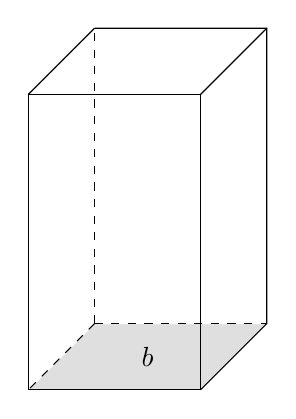
\begin{tikzpicture}[scale=1.25] %add to scale fonts individually ', every node/.style={scale=0.55}]' 
	\def\Width{1.75} 
	\def\Height{3.0} 
	\def\Depth{-1.75}
	\coordinate (O) at (0,0,0);  
	\coordinate (A) at (\Width,0,0);  
	\coordinate (B) at (\Width,\Height,0);  
	\coordinate (C) at (0,\Height,0); 
	\coordinate (D) at (0,0,\Depth);  
	\coordinate (E) at (\Width,0,\Depth);  
	\coordinate (F) at (\Width,\Height,\Depth);  
	\coordinate (G) at (0,\Height,\Depth);
	
	\draw[white, fill=gray!25!white] (O)--(A)--(E)--(D)--cycle;
	\node at (\Width/2,0,\Depth/2) {$b$};
	\fill[opacity=0,text opacity=1] (O) rectangle node {} (B); 
	\draw (O)--(A)--(B)--(C)--(O); 
	\draw[dashed] (D)--(O);  
	\draw[dashed] (D)--(E); 
	\draw[dashed] (D)--(G); 
	\draw(A)--(E)--(F)--(G); 
	\draw (G)--(C); \draw (B)--(F); 
	%%for labels add 'node[pos=.5,below]{$math here$}' after points 
	%% Following is for debugging purposes so you can see where the points are  %% These are last so that they show up on top  
	%%\foreach \xy in {O, A, B, C, D, E, F, G}{  %    \node at (\xy) {\xy}; %} 
\end{tikzpicture}\end{center}
\end{figure}
 \noindent A rectangular prism with a square base $b$ is shown in
the figure. If a plane passing through the rectangular prism is neither
perpendicular nor parallel to the base $b$, which of the following
could be the shape of the intersection of the plane and rectangular
prism?

\begin{itemize}
\item A rectangle with a perimeter less than the perimeter of $b$.
\item A rectangle with a perimeter equal to the perimeter of $b$.
\item [\ansE]A rectangle with a perimeter greater than the perimeter of
$b$.
\item A square with a perimeter less than the perimeter of $b$.
\item A square with a perimeter more than the perimeter of $b$.\yspace \vfill
\end{itemize}
\item \questFill If $-(x+7)=-3(2x+3)-2$, what is the value of $x$? Give
your answer as a fraction.
\[
x=\frac{\,\,\fbox{{ \,}\answer{-4}{ \,}}\,\,}{\fbox{{ \,}\answer{\,5\,}{ \,}}}
\]
\yspace \vfill
\item \questMulti In which of the following are the numbers ordered from
least to greatest?

\begin{itemize}
\item $-\sqrt{2},\frac{2}{5},\frac{2}{9},-2$
\item $-\sqrt{2},-2,\frac{2}{5},\frac{2}{9}$
\item $\frac{2}{5}.\frac{2}{9},-2,-\sqrt{2}$
\item [\ansE]$-2,-\sqrt{2},\frac{2}{9},\frac{2}{5}$
\item $\frac{2}{9},\frac{2}{5},-\sqrt{2},-2$\yspace \vfill
\end{itemize}
\item \questInd If $\frac{2x}{7}$ is between 4 and 6, which of the following
could be the value of $x$?\\
\\
Indicate \textbf{all }that apply.

\begin{itemize}
\item 7
\item 11
\item [\ansB]15
\item [\ansB]19
\item 23\yspace \vfill
\end{itemize}
\item \questMultiPic\renewcommand{\textSize}{\large}
\begin{figure}[H]
\begin{center}\renewcommand{\xmin}{0}
\renewcommand{\xmax}{190}
\renewcommand{\xstep}{0} %must be xmin+n
\renewcommand{\ymax}{55}
\renewcommand{\ymin}{0}
\renewcommand{\ystep}{0} %must be ymin+n
%%%%%%%
\begin{tikzpicture} 
\begin{axis}[height=5.5cm, 
	width=7cm, 
	axis lines=middle,
	xtick={0,30,60,...,180},
	ytick={0,10,20,30,...,40,50},
	minor y tick num={1},
	grid=major,
	xmajorgrids=false,
	axis line style={-latex}, 
	xmin=\xmin,xmax=\xmax, 
	ymin=\ymin,ymax=\ymax,
	every axis x label/.append style={anchor=west}, 
	every axis y label/.append style={anchor=south},
	x label style={at={(axis description cs:0.5,-0.15)},anchor=north},     
	y label style={at={(axis description cs:-0.15,0.5)},rotate=90,anchor=south},
	xlabel={\textSize Total Time in Minutes},
	ylabel={\textSize Total Miles Traveled},
	clip=false, %doesn't clip outside graph
	]
	
	\addplot[mark=*,mark size=2,mark options={solid}, mark indices = {2},thick] coordinates {(30,0) (30,7)} node[anchor=south]{$7$};
	\addplot[mark=*,mark size=2,mark options={solid}, mark indices = {2},thick] coordinates {(60,0) (60,15)} node[anchor=south]{$15$};
	\addplot[mark=*,mark size=2,mark options={solid}, mark indices = {2},thick] coordinates {(90,0) (90,19)} node[anchor=south]{$19$};
	\addplot[mark=*,mark size=2,mark options={solid}, mark indices = {2},thick] coordinates {(120,0) (120,28)} node[anchor=south]{$28$};
	\addplot[mark=*,mark size=2,mark options={solid}, mark indices = {2},thick] coordinates {(150,0) (150,32)} node[anchor=south]{$32$};
	\addplot[mark=*,mark size=2,mark options={solid}, mark indices = {2},thick] coordinates {(180,0) (180,42)} node[anchor=south]{$42$};
	\node[anchor=west] at (axis cs:\xmax,0) {$x$}; \node[anchor=south] at (axis cs:0,\ymax) {$y$};
\end{axis}
\end{tikzpicture}\end{center}
\end{figure}
\noindent Will completed a 42-mile trip in 3 hours. The graph above
indicates the total number of miles Will traveled at 30-minute intervals.
According to the graph, how many miles did Will travel in the last
60 minutes of his trip?

\begin{itemize}
\item 15
\item [\ansE]14
\item 28
\item 35
\item 42\yspace \vfill
\end{itemize}
\item \questMulti\renewcommand{\textSize}{\examTextSize}
\begin{figure}[H]
\begin{center}\renewcommand{\xmin}{-4} 
\renewcommand{\xmax}{8} 
\renewcommand{\xstep}{0} %must be xmin+n 
\renewcommand{\ymin}{-3} 
\renewcommand{\ymax}{5} 
\renewcommand{\ystep}{0} %must be ymin+n

\begin{tikzpicture}  
\begin{axis}[
	height=6cm,
	width=7.5cm,  	
	axis lines=middle, 	
	grid=none, 	
	xmin=\xmin,xmax=\xmax,  	
	ymin=\ymin,ymax=\ymax, 	
	ticks=none, 	
	x label style={at={(axis description cs:0.5,-0.15)},anchor=north},  	y label style={at={(axis description cs:-0.15,0.5)},rotate=90,anchor=south}, 	
	%xlabel={Total Time in Minutes}, 	
	%ylabel={Total Miles Traveled}, 	
	clip=false, %doesn't clip outside graph 	
	]
	
	\addplot[mark=*,mark size=2,mark options={solid}, mark indices = {2},thick] coordinates {(-2,2) (4,-2)} node[anchor=west]{\textSize $B (4,-2)$}; 	
	\addplot[mark=*,mark size=2,mark options={solid}, mark indices = {2},thick] coordinates {(4,-2) (1,4)} node[anchor=west]{\textSize $C (1,4)$}; 	
	\addplot[mark=*,mark size=2,mark options={solid}, mark indices = {2},thick] coordinates {(1,4) (-2,2)} node[anchor=east,align=center]{\textSize $A (-2,2)$}; 	
	\node[anchor=west] at (axis cs:\xmax,0) {$x$};  	
	\node[anchor=south] at (axis cs:0,\ymax) {$y$}; 	
	\node[anchor=north east] at (0,0) {$O$}; 

\end{axis} 
\end{tikzpicture}\end{center}
\end{figure}
\noindent If a triangle $ABC$ in the $xy$-plane shown above is
shifted $7$ units to the right and $4$ units up, what would be the
coordinates of point $A$ after the shift? 

\begin{itemize}
\item $(-5,-6)$
\item $(-5,-2)$
\item $(-5,6)$
\item $(5,-2)$
\item [\ansE]$(5,6)$\yspace \vfill
\end{itemize}
\item \questMultiPic
\begin{figure}[H]
\begin{center}
\[
3.4,3.8,4.2,4.0,3.0,3.9,3.2,3.1,4.7
\]
\end{center}
\end{figure}
 \noindent What is the median of the numbers in the list above?

\begin{itemize}
\item $3.2$
\item $3.4$
\item $3.7$
\item [\ansE]$3.8$
\item $3.9$\yspace \vfill
\end{itemize}
\item \questMulti If $\frac{2}{3}x-7=1$, then $x=$\\


\begin{itemize}
\item 8
\item 9
\item [\ansE]12
\item 16
\item 24\yspace \vfill
\end{itemize}
\item \questInd
\begin{figure}[H]
\begin{center}
\[
\sqrt{18},\alpha,\frac{10}{3},\frac{9}{8},\frac{1}{4},-\sqrt{2}
\]
\end{center}
\end{figure}
 \noindent The five numbers shown are listed in order from \textbf{greatest}
to \textbf{least}. Which of the following could be the value of $\alpha$?\\
\\
Indicate \textbf{all }such values.

\begin{itemize}
\item [\ansB]$\sqrt{17}$
\item $\frac{7}{3}$
\item [\ansB]$\frac{11}{3}$
\item $\frac{23}{8}$
\item $5$\yspace \vfill
\end{itemize}
\item \questMulti Last week Catherine jogged at a constant rate of 4.5
miles per hour from her work to the Happy Jack Hamburger restaurant.
She stayed at the restaurant for 30 minutes and then ran back to work
at a constant rate of 9 miles per hour. If the restaurant is 1.5 mile
from her workplace, which of the following graphs best represents
the relationship between Catherine's distance from work $d$, in miles,
and time $t$, in minutes?


\renewcommand{\textSize}{\large}\begin{multicols}{2}
\begin{itemize}
\item %
\begin{minipage}[c][1\totalheight][t]{1\columnwidth}%
\renewcommand{\xmax}{70}
\renewcommand{\xmin}{0}
\renewcommand{\xstep}{0} %must be xmin+n
\renewcommand{\ymax}{2}
\renewcommand{\ymin}{0}
\renewcommand{\ystep}{0} %must be ymin+n\renewcommand{\xmax}{70}
\renewcommand{\xmin}{0}
\renewcommand{\xstep}{0} %must be xmin+n
\renewcommand{\ymax}{2}
\renewcommand{\ymin}{0}
\renewcommand{\ystep}{0} %must be ymin+n
%%%%%%%
\begin{tikzpicture} 
\begin{axis}[height=4cm, 
	width=6cm, 
	axis lines=middle,
	grid=major,
	xtick={0,10,20,...,60},
	ytick={0,0.5,1.0,1.5},	
	yticklabels={0,1.0,1.5,2.0}, 
	%axis line style={-latex}, 
	xmin=\xmin,xmax=\xmax, 
	ymin=\ymin,ymax=\ymax,
	%restrict y to domain=-1:10,
	no markers, 
	%every axis x label/.append style={anchor=west}, 
	%every axis y label/.append style={anchor=south},
	x label style={at={(axis description cs:0.5,-.25)},anchor=north},     
	y label style={at={(axis description cs:-.275,0.5)},rotate=90,anchor=south},
	xlabel={\textSize Minutes},
	ylabel={\textSize Miles},
	clip=false, %doesn't clip outside graph
	]
	
	\addplot[mark=*,mark size=2,mark options={solid},thick] coordinates {(0,0) (10,1) (40,1) (60,0)} node[anchor=south]{$$};
	\node[anchor=west] at (axis cs:\xmax,0) {$t$}; %\node[anchor=south] at (axis cs:0,\ymax) {$d$};
\end{axis}
\end{tikzpicture}%
\end{minipage}
\item [\ansE]%
\begin{minipage}[c][1\totalheight][t]{1\columnwidth}%
\renewcommand{\xmax}{70} 
\renewcommand{\xmin}{0} 
\renewcommand{\xstep}{0} %must be xmin+n 
\renewcommand{\ymax}{2} 
\renewcommand{\ymin}{0} 
\renewcommand{\ystep}{0} %must be ymin+n %%%%%%% 
\begin{tikzpicture}  
	\begin{axis}[height=4cm,  	
	width=6cm,  	
	axis lines=middle, 	
	grid=major, 	
	xtick={0,10,20,...,60}, 	
	ytick={0,0.5,1.0,1.5}, 	
	yticklabels={0,1.0,1.5,2.0},  	
	%axis line style={-latex},  	
	xmin=\xmin,xmax=\xmax,  	
	ymin=\ymin,ymax=\ymax, 	
	%restrict y to domain=-1:10, 	
	no markers,  	
	%every axis x label/.append style={anchor=west},  	
	%every axis y label/.append style={anchor=south}, 	
	x label style={at={(axis description cs:0.5,-.25)},anchor=north},      		
	y label style={at={(axis description cs:-.275,0.5)},
	rotate=90,anchor=south}, 	
	xlabel={\textSize Minutes}, 	
	ylabel={\textSize Miles}, 	
	clip=false, %doesn't clip outside graph 	
	]
	
	\addplot[mark=*,mark size=2,mark options={solid},thick] coordinates {(0,0) (20,1.0) (50,1) (60,0)} node[anchor=south]{$$};
	\node[anchor=west] at (axis cs:\xmax,0) {$t$}; %\node[anchor=south] at (axis cs:0,\ymax) {$d$};

\end{axis}
\end{tikzpicture}%
\end{minipage}
\item %
\begin{minipage}[c][1\totalheight][t]{1\columnwidth}%
\renewcommand{\xmax}{70} 
\renewcommand{\xmin}{0} 
\renewcommand{\xstep}{0} %must be xmin+n 
\renewcommand{\ymax}{2} 
\renewcommand{\ymin}{0} 
\renewcommand{\ystep}{0} %must be ymin+n %%%%%%% 
\begin{tikzpicture}  
	\begin{axis}[height=4cm,  	
	width=6cm,  	
	axis lines=middle, 	
	grid=major, 	
	xtick={0,10,20,...,60}, 	
	ytick={0,0.5,1.0,1.5}, 	
	yticklabels={0,1.0,1.5,2.0}, 	
	%axis line style={-latex},  	
	xmin=\xmin,xmax=\xmax,  	
	ymin=\ymin,ymax=\ymax, 	
	%restrict y to domain=-1:10, 	
	no markers,  	
	%every axis x label/.append style={anchor=west},  	
	%every axis y label/.append style={anchor=south}, 	
	x label style={at={(axis description cs:0.5,-.25)},anchor=north},      		
	y label style={at={(axis description cs:-.275,0.5)},
	rotate=90,anchor=south}, 	
	xlabel={\textSize Minutes}, 	
	ylabel={\textSize Miles}, 	
	clip=false, %doesn't clip outside graph 	
	]
	
	\addplot[mark=*,mark size=2,mark options={solid},thick] coordinates {(0,0) (20,1.5) (50,1.5) (60,0)} node[anchor=south]{$$};
	\node[anchor=west] at (axis cs:\xmax,0) {$t$}; %\node[anchor=south] at (axis cs:0,\ymax) {$d$};

\end{axis}
\end{tikzpicture}%
\end{minipage}\columnbreak
\item %
\begin{minipage}[c][1\totalheight][t]{1\columnwidth}%
\renewcommand{\xmax}{70} 
\renewcommand{\xmin}{0} 
\renewcommand{\xstep}{0} %must be xmin+n 
\renewcommand{\ymax}{2} 
\renewcommand{\ymin}{0} 
\renewcommand{\ystep}{0} %must be ymin+n %%%%%%% 
\begin{tikzpicture}  
	\begin{axis}[height=4cm,  	
	width=6cm,  	
	axis lines=middle, 	
	grid=major, 	
	xtick={0,10,20,...,60}, 	
	ytick={0,0.5,1.0,1.5}, 	
	yticklabels={0,1.0,1.5,2.0},  	
	%axis line style={-latex},  	
	xmin=\xmin,xmax=\xmax,  	
	ymin=\ymin,ymax=\ymax, 	
	%restrict y to domain=-1:10, 	
	no markers,  	
	%every axis x label/.append style={anchor=west},  	
	%every axis y label/.append style={anchor=south}, 	
	x label style={at={(axis description cs:0.5,-.25)},anchor=north},      		
	y label style={at={(axis description cs:-.275,0.5)},
	rotate=90,anchor=south}, 	
	xlabel={\textSize Minutes}, 	
	ylabel={\textSize Miles}, 	
	clip=false, %doesn't clip outside graph 	
	]
	
	\addplot[mark=*,mark size=2,mark options={solid},thick] coordinates {(0,0) (10,1.5) (40,1.5) (60,0)} node[anchor=south]{$$};
	\node[anchor=west] at (axis cs:\xmax,0) {$t$}; %\node[anchor=south] at (axis cs:0,\ymax) {$d$};

\end{axis}
\end{tikzpicture}%
\end{minipage}
\item %
\begin{minipage}[c][1\totalheight][t]{1\columnwidth}%
\renewcommand{\xmax}{70} 
\renewcommand{\xmin}{0} 
\renewcommand{\xstep}{0} %must be xmin+n 
\renewcommand{\ymax}{2} 
\renewcommand{\ymin}{0} 
\renewcommand{\ystep}{0} %must be ymin+n %%%%%%% 
\begin{tikzpicture}  
	\begin{axis}[height=4cm,  	
	width=6cm,  	
	axis lines=middle, 	
	grid=major, 	
	xtick={0,10,20,...,60}, 	
	ytick={0,0.5,1.0,1.5},	
	yticklabels={0,1.0,1.5,2.0},  	
	%axis line style={-latex},  	
	xmin=\xmin,xmax=\xmax,  	
	ymin=\ymin,ymax=\ymax, 	
	%restrict y to domain=-1:10, 	
	no markers,  	
	%every axis x label/.append style={anchor=west},  	
	%every axis y label/.append style={anchor=south}, 	
	x label style={at={(axis description cs:0.5,-.25)},anchor=north},      		
	y label style={at={(axis description cs:-.275,0.5)},
	rotate=90,anchor=south}, 	
	xlabel={\textSize Minutes}, 	
	ylabel={\textSize Miles}, 	
	clip=false, %doesn't clip outside graph 	
	]
	
	\addplot[mark=*,mark size=2,mark options={solid},thick] coordinates {(0,0) (20,1.0) (40,1.0) (60,0)} node[anchor=south]{$$};
	\node[anchor=west] at (axis cs:\xmax,0) {$t$}; %\node[anchor=south] at (axis cs:0,\ymax) {$d$};

\end{axis}
\end{tikzpicture}%
\end{minipage}\yspace \vfill
\end{itemize}

\end{multicols}

\item \questMulti Which of the following sequences of steps, when completed,
will solve the equation $-3+6z=2$ for $z$?\\


\begin{itemize}
\item Subtract 2 from both sides of the equation, then divide both sides
by $3$.
\item Subtract $2$ from both sides of the equation, then divide both sides
of the new equation by $-3$.
\item Add $3$ to both sides, then subtract $6$ from both sides.
\item [\ansE]Add $3$ to both sides of the equation, then divide both sides
by $6$.
\item Divide both sides of the equation by $6$, then add $3$ to both sides.\yspace \vfill
\end{itemize}
\item \questMulti Last year 55 percent of the total number of sales at
a gas station was for Big Time Chew bubble gum. In which of the following
circle graphs does the shaded area represent the fraction of the total
number of sales which were for Big Time Chew bubble gum?\\



\begin{multicols}{2}
\begin{itemize}
\item %
\begin{minipage}[c][1\totalheight][t]{1\columnwidth}%
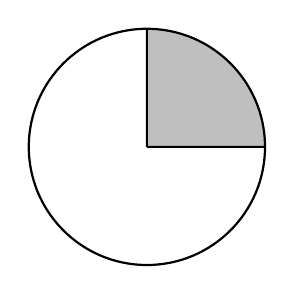
\begin{tikzpicture} 
	\def\Rad{1.5cm};
	\def\End{90};
	\def\Start{0};
	\fill[gray!50!white]   
		(0,0)--(\Start:\Rad) 
		arc[start angle=\Start, 
		end angle =\End,radius=\Rad] --    cycle;
	\draw[color=black,thick]    
		(0,0) circle (\Rad)   	
		(\End:\Rad)--(0,0)   
		(\Start:\Rad)--(0,0); 
\end{tikzpicture}%
\end{minipage}
\item %
\begin{minipage}[c][1\totalheight][t]{1\columnwidth}%
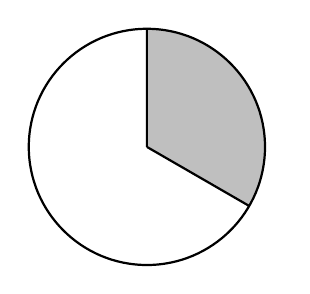
\begin{tikzpicture} 
	\def\Rad{1.5cm};
	\def\End{90};
	\def\Start{-30};
	\fill[gray!50!white]   
		(0,0)--(\Start:\Rad) 
		arc[start angle=\Start, 
		end angle =\End,radius=\Rad] --    cycle;
	\draw[color=black,thick]    
		(0,0) circle (\Rad)   	
		(\End:\Rad)--(0,0)   
		(\Start:\Rad)--(0,0); 
\end{tikzpicture}%
\end{minipage}
\item %
\begin{minipage}[c][1\totalheight][t]{1\columnwidth}%
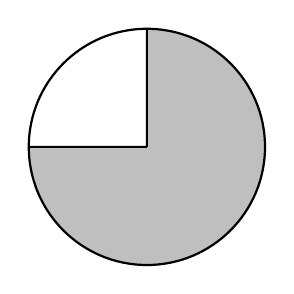
\begin{tikzpicture} 
	\def\Rad{1.5cm};
	\def\End{90};
	\def\Start{-180};
	\fill[gray!50!white]   
		(0,0)--(\Start:\Rad) 
		arc[start angle=\Start, 
		end angle =\End,radius=\Rad] --    cycle;
	\draw[color=black,thick]    
		(0,0) circle (\Rad)   	
		(\End:\Rad)--(0,0)   
		(\Start:\Rad)--(0,0); 
\end{tikzpicture}%
\end{minipage}
\item %
\begin{minipage}[c][1\totalheight][t]{1\columnwidth}%
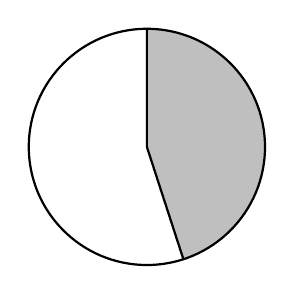
\begin{tikzpicture} 
	\def\Rad{1.5cm};
	\def\End{90};
	\def\Start{-72};
	\fill[gray!50!white]   
		(0,0)--(\Start:\Rad) 
		arc[start angle=\Start, 
		end angle =\End,radius=\Rad] --    cycle;
	\draw[color=black,thick]    
		(0,0) circle (\Rad)   	
		(\End:\Rad)--(0,0)   
		(\Start:\Rad)--(0,0); 
\end{tikzpicture}%
\end{minipage}
\item [\ansE]%
\begin{minipage}[c][1\totalheight][t]{1\columnwidth}%
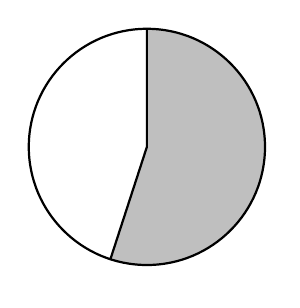
\begin{tikzpicture} 
	\def\Rad{1.5cm};
	\def\End{90};
	\def\Start{-108};
	\fill[gray!50!white]   
		(0,0)--(\Start:\Rad) 
		arc[start angle=\Start, 
		end angle =\End,radius=\Rad] --    cycle;
	\draw[color=black,thick]    
		(0,0) circle (\Rad)   	
		(\End:\Rad)--(0,0)   
		(\Start:\Rad)--(0,0); 
\end{tikzpicture}%
\end{minipage}
\end{itemize}

\end{multicols}\yspace \vfill

\item \questMulti There are 35 people on a  plane, 14 are going to New
York, 11 are going to Salt Lake City, and the rest are going to Asheville.
If one person is randomly selected from the plane, what is the probability
that the person will \textbf{not }be going to New York?\\


\begin{itemize}
\item $\frac{2}{5}$
\item [\ansE]$\frac{3}{5}$
\item $\frac{5}{7}$
\item $\frac{2}{7}$
\item $\frac{24}{35}$\yspace \vfill
\end{itemize}
\item \questMulti The ratio of the number of teachers to the number of
students on a certain field trip was 6 to 24. If the total number
of people on the field trip was 120, how many teachers were on the
tour?\\


\begin{itemize}
\item 20
\item [\ansE]24
\item 30
\item 480
\item 600\yspace \vfill
\end{itemize}
\item \questMulti Wednesday, the temperature was $60^{\circ}$F at 11AM
and $36^{\circ}$F at 3PM. If the temperature fell at a constant rate
from 10AM to 3PM on that day, what was the temperature at 2PM rounded
up to the nearest degree?\\


\begin{itemize}
\item $41^{\circ}$F
\item [\ansE]$42^{\circ}$F
\item $43^{\circ}$F
\item $44^{\circ}$F
\item $45^{\circ}$F\yspace \vfill
\end{itemize}
\item \questMultiPic
\begin{figure}[H]


\[
3s+5p
\]
\end{figure}
\noindent The expression above represents the total amount in yen,
denoted $\yen$, earned by selling $s$ $\mbox{Shopkins}^{\copyright}$
blind bags and $p$ $\mbox{Pokemon}^{\copyright}$ balls. If a Japanese
toy store has a revenue of $\yen644$ by selling both $\mbox{Shopkins}^{\copyright}$
blind bags and $\mbox{Pokemon}^{\copyright}$ balls. The amount earned
by selling $\mbox{Shopkins}^{\copyright}$ blind bags is what fraction
of the total revenue?\\


\begin{itemize}
\item $\frac{s}{644}$
\item $\frac{p}{644}$
\item [\ansE]$\frac{3s}{644}$
\item $\frac{5p}{644}$
\item $\frac{3s+5p}{644}$\yspace \vfill
\end{itemize}
\item \questMultiPic\renewcommand{\textSize}{\examTextSize}
\begin{figure}[H]
\begin{center}\renewcommand{\xmin}{-3.25}
\renewcommand{\xmax}{7.25}
\renewcommand{\xstep}{0} %must be xmin+n
\renewcommand{\ymin}{-6.25}
\renewcommand{\ymax}{2.25}
\renewcommand{\ystep}{0} %must be ymin+n
%%%%%%%
\begin{tikzpicture} 
\begin{axis}[
	scale=1.25,
	height=4.5cm, 
	width=6.5cm, 
	axis lines=middle,
	minor x tick num={1},
	minor y tick num={1},
	grid=both,
	yticklabels={},xticklabels={\empty},
	extra x ticks={-1},extra x tick labels={$-1$},     
	extra y ticks={1},extra y tick labels={$1$},         
	yticklabel style={anchor=west},
	axis line style={-latex}, 
	xmin=\xmin,xmax=\xmax, 
	ymin=\ymin,ymax=\ymax,
	x label style={at={(axis description cs:0.5,-0.15)},anchor=north},     
	y label style={at={(axis description cs:-0.15,0.5)},rotate=90,anchor=south},
	clip=false, %doesn't clip outside graph
	]

	\def\Apt{(5,-1)};
	\def\Bpt{(2,-4)};
	\def\Cpt{(2,-1)};
	
	\addplot[mark=*,mark size=2,mark options={solid}, mark indices = {2},thick] coordinates {\Cpt \Apt} node[anchor=west]{\textSize $A$};
	\addplot[mark=*,mark size=2,mark options={solid}, mark indices = {2},thick] coordinates {\Apt \Bpt} node[anchor=north east]{\textSize $B$};
	\addplot[mark=*,mark size=2,mark options={solid}, mark indices = {2},thick] coordinates {\Bpt \Cpt} node[anchor=east]{\textSize $C$};
	%\node[anchor=west] at (axis cs:\xmax,0) {$x$}; \node[anchor=south] at (axis cs:0,\ymax) {$y$};
	%\node[anchor=south east] at (0,0) {$O$};
\end{axis}
\end{tikzpicture}\end{center}
\end{figure}
\noindent Triangle $ABC$ in the $xy$-plane above will be translated
2 units to the left and then 4 units up. What point will correspond
to vertex $A$ after these translations?\\


\begin{itemize}
\item $(-1,-1)$
\item $(1,1)$
\item $(1,5)$
\item [\ansE]$(3,3)$
\item $(3,5)$\yspace \vfill
\end{itemize}
\item \questMultiPic
\begin{figure}[H]
\[
60.5,56.5,56,62,58,57,55.5,63,59.5,61.5,56
\]
\end{figure}
\noindent Max ran the 400-meter 11 times in competitions during the
spring track season. His times, in seconds, are listed above. What
is the mid-range of Max's times, in seconds?\\


\begin{itemize}
\item 7
\item 7.5
\item 58.68
\item 59
\item [\ansE]59.25\yspace \vfill
\end{itemize}
\item \questMultiPic
\begin{figure}[H]
\begin{center}

NUMBER OF PIES SOLD\vspace{5pt}

\begin{tabular}{|l|ccccc|}
\hline 
Chocolate & \faBirthdayCake & \faBirthdayCake & \faBirthdayCake & \faBirthdayCake & \faBirthdayCake\tabularnewline
\hline 
Vanilla & \faBirthdayCake & \faBirthdayCake & \faBirthdayCake &  & \tabularnewline
\hline 
Carrot & \faBirthdayCake & \faBirthdayCake & \faBirthdayCake & \faBirthdayCake & \tabularnewline
\hline 
\end{tabular}\end{center}

\caption*{Each \faBirthdayCake~represents 8 cakes.}
\end{figure}
\noindent The pictograph above shows the number of cakes sold one
day at Charlie's Cake Factory. Chocolate cakes sell for $\$10.50$
each, vanilla cakes cost for $\$10.00$ each, and the total sales
of the all three types of pies was $\$1,012.00$. How much does a
carrot pie cost?\\


\begin{itemize}
\item \$10.25
\item \$10.50
\item [\ansE]\$11.00
\item \$11.25
\item \$11.50\yspace \vfill
\end{itemize}
\item \questMultiPic
\begin{figure}[H]
\begin{center}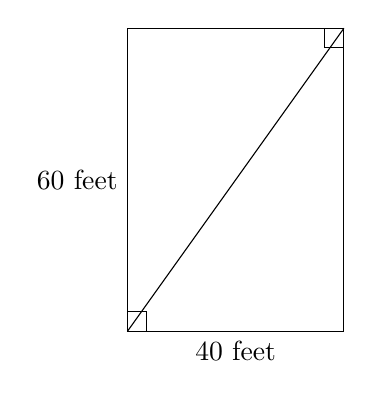
\begin{tikzpicture}[scale=.55]
	\coordinate (A) at (0,0); 
	\coordinate (B) at (0,7); 
	\coordinate (C) at (5,7);
	\coordinate (D) at (5,0);
	%note I should try to do all tkz-euclide here for labels
	\draw (A) node[anchor=north east]{$$}
	--(B) node[anchor=east, pos=.5]{60 feet}
	--(C)    
	--(D) --cycle node[anchor=north, pos=.5]{40 feet}; 
	
	\draw (A)--(C);
	
	\tkzMarkRightAngle[size=0.45,opacity=1](D,A,B)
	\tkzMarkRightAngle[size=0.45,opacity=1](B,C,D)

\end{tikzpicture} \end{center}
\end{figure}
\noindent A farmer wants to build a diagonal fence that will divide
her pig pen. The pig pen is 40 feet wide and 60 feet long, as shown
in the figure. Approximately what is the length, in feet, of the diagonal
brace?\\


\begin{itemize}
\item 55 feet
\item 65 feet
\item [\ansE]75 feet
\item 85 feet
\item 95 feet\yspace \vfill
\end{itemize}
\item \questMultiPic \renewcommand{\textSize}{large} \Large
\begin{figure}[H]
\begin{center}\renewcommand{\xmin}{0}
\renewcommand{\xmax}{75}
\renewcommand{\xstep}{0} %must be xmin+n
\renewcommand{\ymin}{0}
\renewcommand{\ymax}{96}
\renewcommand{\ystep}{0} %must be ymin+n
%%%%%%%
\begin{tikzpicture} 
\begin{axis}[
	height=5.5cm, 
	width=5.5cm, 
	axis lines=middle,
	%minor x tick num={1},
	%minor y tick num={1},
	grid=major,
	%xmajorgrids=false,
	xtick={0,14,28,...,70},
	ytick={0,9,18,...,81},
	axis line style={-latex}, 
	xmin=\xmin,xmax=\xmax, 
	ymin=\ymin,ymax=\ymax,
	clip=false, %doesn't clip outside graph
	]
	\addplot[domain=\xmin-2:\xmax-2,thick]{-15/14*x+75} node[anchor=south]{$$};	
	\node[anchor=west] at (axis cs:\xmax,0) {$x$}; \node[anchor=south] at (axis cs:0,\ymax) {$y$};
\end{axis}
\end{tikzpicture}\end{center}
\end{figure}
\renewcommand{\textSize}{\examTextSize} \examTextSize \noindent The
graph of the linear equation is shown in the $xy$-plane above. Which
of the following tables of values from linear equations rounded to
the nearest tenth corresponds to the graph?


\begin{multicols}{3}
\begin{itemize}
\item %
\begin{tabular}{|r|l|}
\hline 
$x$ & $y$\tabularnewline
\hline 
28 & 45\tabularnewline
\hline 
42 & 31\tabularnewline
\hline 
56 & 17\tabularnewline
\hline 
70 & 3\tabularnewline
\hline 
\end{tabular}
\item %
\begin{tabular}{|r|l|}
\hline 
$x$ & $y$\tabularnewline
\hline 
28 & 44.4\tabularnewline
\hline 
42 & 29.6\tabularnewline
\hline 
56 & 14.8\tabularnewline
\hline 
70 & 0\tabularnewline
\hline 
\end{tabular}
\item %
\begin{tabular}{|r|l|}
\hline 
$x$ & $y$\tabularnewline
\hline 
28 & 45\tabularnewline
\hline 
42 & 33\tabularnewline
\hline 
56 & 21\tabularnewline
\hline 
70 & 9\tabularnewline
\hline 
\end{tabular}
\item [\ansE]%
\begin{tabular}{|r|l|}
\hline 
$x$ & $y$\tabularnewline
\hline 
28 & 45\tabularnewline
\hline 
42 & 30\tabularnewline
\hline 
56 & 15\tabularnewline
\hline 
70 & 0\tabularnewline
\hline 
\end{tabular}
\item %
\begin{tabular}{|r|l|}
\hline 
$x$ & $y$\tabularnewline
\hline 
28 & 42\tabularnewline
\hline 
42 & 26\tabularnewline
\hline 
56 & 10\tabularnewline
\hline 
70 & -6\tabularnewline
\hline 
\end{tabular}
\end{itemize}

\end{multicols}\yspace \vfill

\item \questMulti An administrator at a state university wants to find
out how students feel about raising parking fees to pay for a new
student athletic center. Which of the following methods of selecting
the sample will yield the most valid information about the feelings
of all the students at the university?

\begin{itemize}
\item Interviewing students on campus at random between classes on Monday.
\item Randomly choosing forty students from the library on a given day.
\item Selecting a random sample of freshmen.
\item [\ansE]Selecting a random sample from a list of all students currently
enrolled at the school.
\item Sending a questionnaire to all students and using the returned questionnaires
as the sample.\yspace \vfill
\end{itemize}
\item \questMultiPic \renewcommand{\textSize}{\small}
\begin{figure}[H]
\begin{center}%%draw regular polygon
%%requires \usepackage{luamplib}%%%	
%\begin{mplibcode}   
	%beginfig(1);     
	%u = 3cm; n = 5; angl = 360/n;     
	%% The regular polygon at the center     
	%z0 = u*dir(-90 - .5angl);     
	%path polygon;      
	%polygon = z0 for i = 1 upto n-1: hide(z[i] = z[i-1] rotated angl) -- z[i] endfor -- cycle;     
	%% Drawing the other polygons 
	%for i = 0 upto n-1: draw polygon rotatedaround (z[i], 180-angl); 
	%endfor;   
	%endfig; 
%\end{mplibcode}

%%%using tikz%%%%
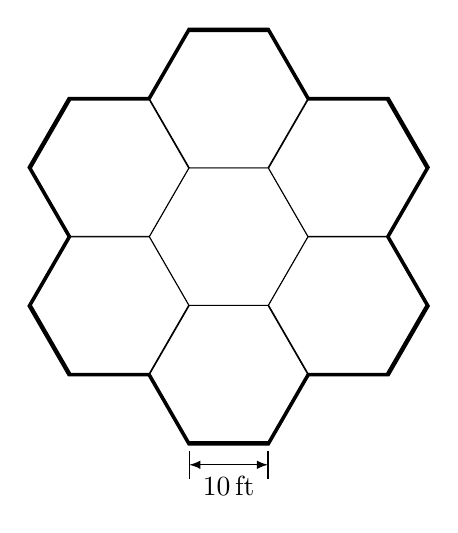
\begin{tikzpicture}[scale=1.0]   
\tkzDefPoint(-.5,-1.75){A}
\tkzDefPoint(.5,-1.75){B}

%thick outside
\tikzset{pntgn/.style={regular polygon, regular polygon sides=6,draw,ultra thick,minimum size=2cm,anchor=south}}   
	\node(n)[pntgn,draw=none,outer sep=0pt]{};   
	\foreach\deg[count=\x] in{0,60,...,300}{\node[pntgn,rotate=\deg,at=(n.side \x)]{};
}
	
%thin inside
\tikzset{pntgn/.style={fill=white,regular polygon, regular polygon sides=6,draw, minimum size=2cm,anchor=south}}   
	\node(n)[pntgn,draw=none,outer sep=0pt]{};   
	\foreach\deg[count=\x] in{0,60,...,300}{\node[pntgn,rotate=\deg,at=(n.side \x)]{};
} 
	%%node at end
	%..\foreach list should be {0,60,...,300} instead, because 
	%side 1 corresponds to rotation=0, side 2 to rotation=60, ... and side 6 to rotation=300
	%example pentagons= \foreach\deg[count=\x] in{36,108,...,324}

\foreach \Nodo in {A,B}            
		\draw([yshift=-3pt]\Nodo)-- ([yshift=-13pt]\Nodo);
		\draw[<->,>=latex] ([yshift=-8pt]A) -- node[yshift=-7.5pt] {\textSize $10$\,ft} ([yshift=-8pt]B);

\end{tikzpicture}\end{center}
\end{figure}
 \noindent \renewcommand{\textSize}{examTextSize}A large platform
is constructed of 7 congruent pieces, each of which is the shape of
a right prism with regular hexagon bases that have sides 10 feet long.
If the platform is 5 feet tall, which of the following best approximates
the volume of the entire platform? (The area of a hexagon with side
length $a$ is approximately $2.6a^{2}$.)

\begin{itemize}
\item 1,300 cubic feet 
\item 910 cubic feet
\item 1,820 cubic feet
\item [\ansE]9,100 cubic feet
\item 4,320 cubic feet\yspace \vfill
\end{itemize}
\item \questMultiPic\renewcommand{\textSize}{\large}
\begin{figure}[H]
\begin{center}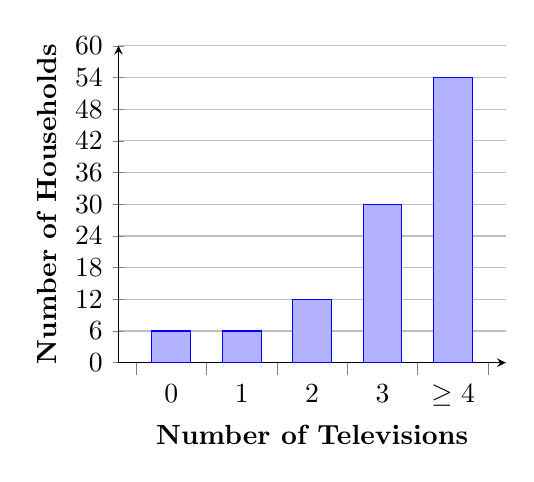
\begin{tikzpicture} 
\begin{axis}[
	%scale=.65,
	width=6.5cm,
	axis lines=left,
	enlarge x limits=0.05, 
	legend style={at={(0.5,-0.15)},anchor=north,legend columns=-1 }, 
	ymin=0, 
	ybar interval=.55, 
	xtick=data,
	ytick={0,6,12,...,66},
	%y tick label style={/pgf/number format/fixed},
	xticklabel style={text width=20pt, align=center,font=\textSize},
	yticklabel style={font=\textSize},
	%scaled y ticks = false,
	%yticklabels={0,500000,1000000,1500000},
	%symbolic x coords={0,1,2,3,4,5}, 
	xticklabels={0,1,2,3, $\geq 4$},
	ylabel=\textSize \textbf{Number of Households},
	xlabel=\textSize \textbf{Number of Televisions},
	grid=major,
	xmajorgrids=false,
	clip=false, 
	tick pos=left] 	

	\addplot coordinates {(0,6) (1,6) (2,12) (3,30) (4,54) (5,60)}; 
	%\legend{0-10,10-20,20-30,$>30$} 
\end{axis} 

\end{tikzpicture}\end{center}
\end{figure}
 \noindent A survey of 108 randomly selected households was conducted.
The graph above shows the number of households with either 0, 1, 2,
3, or 4 or more televisions. How many of the 108 households had at
least 2 televisions? 

\begin{itemize}
\item 12
\item 24
\item 48
\item 84
\item [\ansE]96\yspace \vfill
\end{itemize}
\item \questFill Alex works for an insurance firm. He earns \$1050 per
month plus \$525 for each insurance policy that he sells that month.
If he wants to earn more than \$6300 this month, what is the minimum
number of insurance policies that he must sell this month?
\begin{figure}[H]
\begin{center}
\[
\fbox{{\ensuremath{\begin{array}{cc}
 \,  &  \answer{11} \,\,\end{array}}}}\mbox{ insurance policies}
\]
\end{center}
\end{figure}
 \yspace \vfill
\item \questMulti Which of the following scatterplots most strongly suggests
a positive linear relationship between $x$ and $y$?


\begin{multicols}{2}
\begin{itemize}
\item %
\begin{minipage}[c][1\totalheight][t]{1\columnwidth}%
%%%%%%% 
\renewcommand{\xmin}{-10}
\renewcommand{\xmax}{16}
\renewcommand{\ymin}{-5}
\renewcommand{\ymax}{16}

\begin{tikzpicture} 
\begin{axis}[
	scale=.5,
	scatter/classes={a={mark=o,draw=black}},
	xmin=\xmin, xmax=\xmax,
	ymin=\ymin, ymax=\ymax,
	xtick={10},
	ytick={10},
	xticklabels={},yticklabels={},
	extra x ticks={},extra y ticks={},
	extra x tick style={xticklabel=\pgfmathprintnumber{\tick}},
	extra y tick style={yticklabel=\pgfmathprintnumber{\tick},y tick label style={right}},
	axis lines=middle,
	axis line style = thick,
	clip=false
	] 

\addplot [scatter,only marks,scatter src=explicit symbolic,mark size=1.5,xshift=0cm]
table[] { 
x y label 
2.5376592	13.910799 
4.9517813	13.696123 
6.242109	12.889044 
3.6075575	11.428853 
5.3361692	9.302227 
8.28138	10.842657 
7.239338	9.745053 
5.468639	7.2799115 
7.569679	7.2962623 
9.236068	8.165261 
10.631917	8.798692 
10.800872	7.0879445 
12.213071	5.620335 
13.702481	4.231148 
11.5318	3.1636715 
10.08039	4.669886 
7.6309934	4.4173617 
	};

\node[anchor=west] at (axis cs:\xmax,0) {$x$};
\node[anchor=south] at (axis cs:0,\ymax) {$y$};
%\node[anchor=north east] at (axis cs:0,0) {$O$};

\end{axis}
\end{tikzpicture}%
\end{minipage}
\item %
\begin{minipage}[c][1\totalheight][t]{1\columnwidth}%
%%%%%%% 
\renewcommand{\xmax}{16}
\renewcommand{\ymax}{16}
\renewcommand{\xmin}{-10}
\renewcommand{\ymin}{-5}
\begin{tikzpicture} 
\begin{axis}[
	scale=.5,
	scatter/classes={a={mark=o,draw=black}},
	xmin=\xmin, xmax=\xmax,
	ymin=\ymin, ymax=\ymax,
	xtick={},
	ytick={},
	xticklabels={},yticklabels={},
	extra x ticks={},extra y ticks={},
	extra x tick style={xticklabel=\pgfmathprintnumber{\tick}},
	extra y tick style={yticklabel=\pgfmathprintnumber{\tick},y tick label style={left}},
	axis lines=middle,
	axis line style = thick,
	clip=false
	] 
\addplot[scatter,only marks,scatter src=explicit symbolic,mark size=1.5,xshift=1.25cm]
table[] { 
x y label 
-5.726984	14.190513 
-6.2844253	11.873288 
-3.2969267	12.560281 
-1.8534606	10.556097 
-4.027355	10.562398 
-5.1066155	8.2177 
-1.6308202	7.367046 
-3.4326954	5.7200947 
-0.9409709	5.3650465 
-1.8742124	3.3967369 
1.8690875	4.835162 
2.0962646	3.2113152 
4.5947104	5.175088 
3.5281367	7.207165 
5.296826	7.404937 
5.766135	9.31662 
7.4756775	9.108767 
6.4391813	11.517568 
9.052812	13.220137 
	};
\node[anchor=west] at (axis cs:\xmax,0) {$x$};
\node[anchor=south] at (axis cs:0,\ymax) {$y$};
%\node[anchor=north east] at (axis cs:0,0) {$O$};

\end{axis}
\end{tikzpicture}%
\end{minipage}
\item %
\begin{minipage}[c][1\totalheight][t]{1\columnwidth}%
%%%%%%% 
\renewcommand{\xmin}{-10}
\renewcommand{\xmax}{16}
\renewcommand{\ymax}{5}
\renewcommand{\ymin}{-16}
\begin{tikzpicture} 
\begin{axis}[
	scale=.5,
	scatter/classes={a={mark=o,draw=black}},
	xmin=\xmin, xmax=\xmax,
	ymin=\ymin, ymax=\ymax,
	xtick={10},
	ytick={10},
	xticklabels={},yticklabels={},
	extra x ticks={},extra y ticks={10},
	extra x tick style={xticklabel=\pgfmathprintnumber{\tick}},
	extra y tick style={yticklabel=\pgfmathprintnumber{\tick}},
	axis lines=middle,
	axis line style = thick,
	clip=false
	] 
\addplot[scatter,only marks,scatter src=explicit symbolic,mark size=1.5,yshift=-2cm]
table[] { 
x y label 
-2.190597	2.160066 
-4.2989573	2.6014109 
-2.6291103	4.6482167 
-3.4459367	6.0459933 
-1.5520319	6.164547 
1.8659592	9.100814 
1.6078001	10.888475 
1.247584	12.219281 
3.4224231	12.304719 
5.3318396	10.212855 
3.7633111	8.728164 
6.224747	7.973507 
8.15817	7.460759 
5.60945	5.6533995 
7.328171	5.735636 
8.248778	4.549114 
9.726083	4.0331655 
7.419764	2.6836474 
	};
\node[anchor=west] at (axis cs:\xmax,0) {$x$};
\node[anchor=south] at (axis cs:0,\ymax) {$y$};
%\node[anchor=north east] at (axis cs:0,0) {$O$};

\end{axis}
\end{tikzpicture}%
\end{minipage}
\item [\ansE]%
\begin{minipage}[c][1\totalheight][t]{1\columnwidth}%
%%%%%%% 
\renewcommand{\xmin}{-16}
\renewcommand{\xmax}{10}
\renewcommand{\ymin}{-16}
\renewcommand{\ymax}{5}
\begin{tikzpicture} 
\begin{axis}[
	scale=.5,
	scatter/classes={a={mark=o,draw=black}},
	xmin=\xmin, xmax=\xmax,
	ymin=\ymin, ymax=\ymax,
	xtick={10},
	ytick={10},
	xticklabels={},yticklabels={},
	extra x ticks={},extra y ticks={},
	extra x tick style={xticklabel=\pgfmathprintnumber{\tick}},
	extra y tick style={yticklabel=\pgfmathprintnumber{\tick}},
	extra y tick style={yticklabel=\pgfmathprintnumber{\tick},y tick label style={right}},
	axis lines=middle,
	axis line style = thick,
	clip=false
	] 
\addplot[scatter,only marks,scatter src=explicit symbolic,mark size=1.5,yshift=-2cm]
table[] { 
x y label 
-12.517043	2.3232613 
-10.150206	2.5083032 
-8.845923	3.3963041 
-11.501311	4.8710203 
-9.77725	6.961918 
-7.7615185	6.5096765 
-6.7333	5.5239105 
-4.408041	7.4755898 
-5.7888627	8.2480955 
-7.558247	8.983893 
-9.642901	8.941191 
-7.604195	11.987265 
-5.0589337	11.678237 
-4.308778	9.384068 
-2.8651516	10.837933 
-1.4211512	12.185791 
-3.474591	13.309278  
	};
\node[anchor=west] at (axis cs:\xmax,0) {$x$};
\node[anchor=south] at (axis cs:0,\ymax) {$y$};
%\node[anchor=north east] at (axis cs:0,0) {$O$};

\end{axis}
\end{tikzpicture}%
\end{minipage}
\item %
\begin{minipage}[c][1\totalheight][t]{1\columnwidth}%
%%%%%%% 
\renewcommand{\xmax}{16}
\renewcommand{\ymax}{16}
\renewcommand{\xmin}{-10}
\renewcommand{\ymin}{-5}
\begin{tikzpicture} 
\begin{axis}[
	scale=.5,
	scatter/classes={a={mark=o,draw=black}},
	xmin=\xmin, xmax=\xmax,
	ymin=\ymin, ymax=\ymax,
	xtick={10},
	ytick={10},
	xticklabels={},yticklabels={},
	extra x ticks={},extra y ticks={},
	extra x tick style={xticklabel=\pgfmathprintnumber{\tick}},
	extra y tick style={yticklabel=\pgfmathprintnumber{\tick}},
	axis lines=middle,
	axis line style = thick,
	clip=false
	] 
\addplot[scatter,only marks,scatter src=explicit symbolic,mark size=1.5,yshift=1cm]
table[] { 
x y label 
1.5895656	4 
3.6857862	4 
5.737958	4 
7.7466536	4 
9.842684	4 
11.807902	4 
14.034743	4 
	};
\node[anchor=west] at (axis cs:\xmax,0) {$x$};
\node[anchor=south] at (axis cs:0,\ymax) {$y$};
%\node[anchor=north east] at (axis cs:0,0) {$O$};

\end{axis}
\end{tikzpicture}%
\end{minipage}
\end{itemize}

\end{multicols}\yspace \vfill

\item \questMulti If $a+b=10$ and $c+d=20$, what is the value of $(5a+5b)(3c+3d)?$

\begin{itemize}
\item 2,000
\item [\ansE]3,000
\item 6,000
\item 10,000
\item 12,000\yspace \vfill
\end{itemize}
\item \questMulti Robin sets up a conversion as follows:
\begin{figure}[H]
\begin{center}
\[
5\mbox{ miles}\times\frac{1,609,344\mbox{ meters}}{1\mbox{000 mile}}\times\frac{100\mbox{ centimeters}}{1\mbox{ meter}}
\]
\end{center}
\end{figure}
 \noindent Which one of the following conversions is she performing?

\begin{itemize}
\item [\ansE]Miles to centimeters
\item Miles to meters 
\item Meters to miles
\item Centimeters to miles
\item Miles to 1000 centimeters\yspace \vfill
\end{itemize}
\item \questMulti A painter needs to paint 4 houses, each having an area
of approximately 1,450 square feet. If the brand of paint he plans
to purchase covers 300 square feet per gallon, what is the minimum
number of gallons he needs to purchase?

\begin{itemize}
\item 4
\item 5
\item 19
\item [\ansE]20
\item 5,800\yspace \vfill
\end{itemize}
\item \questMulti Each of the following dot plots represents a distribution
of 16 values. In which distribution is the mean less than the median?

\begin{itemize}
\item %
\begin{minipage}[c][1\totalheight][t]{1\columnwidth}%
%%%%%%% 
\renewcommand{\xmin}{-.5}
\renewcommand{\xmax}{6.5}
\renewcommand{\ymin}{0}
\renewcommand{\ymax}{3}
\begin{tikzpicture} 
\begin{axis}[
	hide y axis,
	width=6cm, height=2.5cm,
	scale=1.0,
	scatter/classes={a={mark=o,draw=black}},
	xmin=\xmin, xmax=\xmax,
	ymin=\ymin, ymax=\ymax,
	xtick={0,1,2,3,4,5,6},
	xticklabels={0,1,2,3,4,5,6},
	axis lines*=left,
	axis line style = thick,
	clip=false
	] 
\addplot[scatter,only marks,scatter src=explicit symbolic,mark size=1.5]
table[] { 
x y label 
0	1
1	1
1	2
2	1
2	2
2	3
3	1
3	2
3	3
3	4
4	1
4	2
4	3
5	1
5	2
6	1
	};
\node[anchor=west] at (axis cs:\xmax,0) {$x$};
%\node[anchor=south] at (axis cs:0,\ymax) {$y$};

\end{axis}
\end{tikzpicture} %
\end{minipage}
\item %
\begin{minipage}[c][1\totalheight][t]{1\columnwidth}%
%%%%%%% 
\renewcommand{\xmin}{-.5}
\renewcommand{\xmax}{6.5}
\renewcommand{\ymin}{0}
\renewcommand{\ymax}{3}
\begin{tikzpicture} 
\begin{axis}[
	hide y axis,
	width=6cm, height=2.5cm,
	scale=1.0,
	scatter/classes={a={mark=o,draw=black}},
	xmin=\xmin, xmax=\xmax,
	ymin=\ymin, ymax=\ymax,
	xtick={0,1,2,3,4,5,6},
	xticklabels={0,1,2,3,4,5,6},
	axis lines*=left,
	axis line style = thick,
	clip=false
	] 
\addplot[scatter,only marks,scatter src=explicit symbolic,mark size=1.5]
table[] { 
x y label 
0	1
1	1
1	2
2	1
2	2
2	3
3	1
3	2
3	3
3	4
4	1
4	2
4	3
5	1
6	1
6	2
	};
\node[anchor=west] at (axis cs:\xmax,0) {$x$};
%\node[anchor=south] at (axis cs:0,\ymax) {$y$};

\end{axis}
\end{tikzpicture}%
\end{minipage}
\item [\ansE]%
\begin{minipage}[c][1\totalheight][t]{1\columnwidth}%
%%%%%%% 
\renewcommand{\xmin}{-.5}
\renewcommand{\xmax}{6.5}
\renewcommand{\ymin}{0}
\renewcommand{\ymax}{3}
\begin{tikzpicture} 
\begin{axis}[
	hide y axis,
	width=6cm, height=2.5cm,
	scale=1.0,
	scatter/classes={a={mark=o,draw=black}},
	xmin=\xmin, xmax=\xmax,
	ymin=\ymin, ymax=\ymax,
	xtick={0,1,2,3,4,5,6},
	xticklabels={0,1,2,3,4,5,6},
	axis lines*=left,
	axis line style = thick,
	clip=false
	] 
\addplot[scatter,only marks,scatter src=explicit symbolic,mark size=1.5]
table[] { 
x y label 
0	1
0	2
1	1
2	1
2	2
2	3
3	1
3	2
3	3
3	4
4	1
4	2
4	3
5	1
5	2
6	1
	};
\node[anchor=west] at (axis cs:\xmax,0) {$x$};
%\node[anchor=south] at (axis cs:0,\ymax) {$y$};

\end{axis}
\end{tikzpicture}%
\end{minipage}
\item %
\begin{minipage}[c][1\totalheight][t]{1\columnwidth}%
%%%%%%% 
\renewcommand{\xmin}{-.5}
\renewcommand{\xmax}{6.5}
\renewcommand{\ymin}{0}
\renewcommand{\ymax}{3}
\begin{tikzpicture} 
\begin{axis}[
	hide y axis,
	width=6cm, height=2.5cm,
	scale=1.0,
	scatter/classes={a={mark=o,draw=black}},
	xmin=\xmin, xmax=\xmax,
	ymin=\ymin, ymax=\ymax,
	xtick={0,1,2,3,4,5,6},
	xticklabels={0,1,2,3,4,5,6},
	axis lines*=left,
	axis line style = thick,
	clip=false
	] 
\addplot[scatter,only marks,scatter src=explicit symbolic,mark size=1.5]
table[] { 
x y label 
0	1
0	2
1	1
2	1
2	2
2	3
3	1
3	2
3	3
3	4
4	1
4	2
4	3
5	1
6	1
6	2
	};
\node[anchor=west] at (axis cs:\xmax,0) {$x$};
%\node[anchor=south] at (axis cs:0,\ymax) {$y$};

\end{axis}
\end{tikzpicture}%
\end{minipage}
\item %
\begin{minipage}[c][1\totalheight][t]{1\columnwidth}%
%%%%%%% 
\renewcommand{\xmin}{-.5}
\renewcommand{\xmax}{6.5}
\renewcommand{\ymin}{0}
\renewcommand{\ymax}{3}
\begin{tikzpicture} 
\begin{axis}[
	hide y axis,
	width=6cm, height=2.5cm,
	scale=1.0,
	scatter/classes={a={mark=o,draw=black}},
	xmin=\xmin, xmax=\xmax,
	ymin=\ymin, ymax=\ymax,
	xtick={0,1,2,3,4,5,6},
	xticklabels={0,1,2,3,4,5,6},
	axis lines*=left,
	axis line style = thick,
	clip=false
	] 
\addplot[scatter,only marks,scatter src=explicit symbolic,mark size=1.5]
table[] { 
x y label 
2	1
2	2
2	3
2	4
3	1
3	2
3	3
3	4
4	1
4	2
4	3
4	4
5	1
5	2
5	3
5	4
	};
\node[anchor=west] at (axis cs:\xmax,0) {$x$};
%\node[anchor=south] at (axis cs:0,\ymax) {$y$};

\end{axis}
\end{tikzpicture}%
\end{minipage}\yspace \vfill
\end{itemize}
\item \questMulti $A$ is one-half as much as $B$, and $B$ is 2 more
than 10 times $C$. Which of the following statements describes the
relationship between $A$ and $C$?

\begin{itemize}
\item $A$ is 2 more than 20 times $C$.
\item $A$ is 4 more than 20 times $C$.
\item $A$ is 4 more than 5 times $C$.
\item [\ansE]$A$ is 1 more than 5 times $C$.
\item $A$ is 1 less than 5 times $C$.\yspace \vfill
\end{itemize}
\item \questMulti A charity has $\$30,000$ available to spend on a fundraiser
ball. The total cost $t,$ in dollars, for the fundraiser is estimated
by the equation $t=390g+7,800$ where $g$ is the number of guests.
What is the maximum number of quests that can attend the fundraiser
ball?

\begin{itemize}
\item [\ansE]56
\item 57
\item 76
\item 77
\item 96\yspace \vfill
\end{itemize}
\item \questMulti Of the following, which is the most likely to be the
height of an adult man?

\begin{itemize}
\item 1 meter
\item 3 feet 
\item 132 inches
\item 150 centimeters
\item [\ansE]2000 millimeters\yspace \vfill
\end{itemize}
\item \questMulti A bag contains a number of solid-colored marbles. 13
of the marbles are blue, 5 of the marbles are yellow, and the rest
are red. If a person were to randomly draw a marble from the bag,
the probability that the marble drawn would be yellow is $\frac{1}{5}$.
How many red marbles are in the bag?

\begin{itemize}
\item 5
\item 6
\item [\ansE]7
\item 8
\item 9\yspace \vfill
\end{itemize}
\item \questMulti The price of a calculator was increased from $\$90$
to $\$138$ just before the start of school. By approximately what
percent was the price of the calculator increased?

\begin{itemize}
\item $35\%$
\item $48\%$
\item [\ansE]$53\%$
\item $65\%$
\item $153\%$\yspace \vfill
\end{itemize}
\item \questMultiPic \renewcommand{\textSize}{\examTextSize}
\begin{figure}[H]
%%%%%%% 
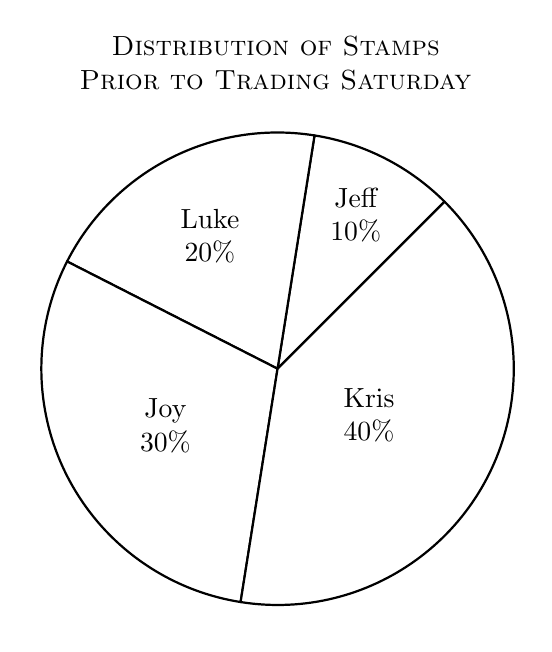
\begin{tikzpicture}[font=\textSize]
	\pie[text = inside,color=white,rotate=45]{10/Jeff , 20/Luke , 30/Joy , 40/Kris} 
	\node[align=center, yshift=2em,font=\textSize] (title)      at (current bounding box.north)	{\textsc{Distribution of Stamps} \\ \textsc{Prior to Trading Saturday}};
\end{tikzpicture}
%%%see package options: 
%%%http://ctan.math.washington.edu/tex-archive/graphics/pgf/contrib/pgf-pie/pgf-%%%pie-manual.pdf
%%%note this package may create conflicts with others that define 'text'. fx by %%%redefining 'text' as 'textASDF' or something in the .sty file.

\end{figure}
\renewcommand{\textSize}{\examTextSize} \noindent Kris, Jeff, Luke,
and Joy collect stamps. Collectively they have a total of 550 stamps.
Every Saturday they get together and trade stamps. The pie chart above
shows the distribution of the 550 stamps before trading. At the end
of trading Saturday night, Kris has 18 percent, Luke 30 percent, and
Joy has 28 percent of the total number of stamps. How many more stamps
does Jeff have at the end of trading than he had before the trading
began?

\begin{itemize}
\item 14
\item 24
\item 66
\item [\ansE]77
\item 99\yspace \vfill
\end{itemize}
\item \questMulti Jim has a big wheelbarrow with a wheel 20 inches in diameter,
and his son, James, has a little wheelbarrow with a wheel 10 inches
in diameter. Jim pushes his big wheelbarrow straight across a filed
so that the wheel makes 150 revolutions. If James follows Jim and
pushes his wheelbarrow the same distance, how many revolutions will
the wheel of the little wheelbarrow turn?

\begin{itemize}
\item 75
\item 75$\pi$
\item 150
\item [\ansE]300
\item 300$\pi$\yspace \vfill
\end{itemize}
\item \questFill Suppose that there are five children at a birthday party.
The ages of the first four children are 5, 9, 4, and 3. If the mean
of the children is 6, how old is the fifth child?
\begin{figure}[H]
\begin{center}
\[
x=\fbox{{\ensuremath{\begin{array}{cc}
 \,  &  \answer{9} \,\,\end{array}}}}\mbox{ years old}
\]
\end{center}
\end{figure}
\yspace \vfill
\item \questMultiPic 
\begin{figure}[H]
\begin{center}\renewcommand{\xmax}{35}
\renewcommand{\xmin}{0}
\renewcommand{\xstep}{0} %must be xmin+n
\renewcommand{\ymax}{74}
\renewcommand{\ymin}{0}
\renewcommand{\ystep}{0} %must be ymin+n
%%%%%%%
\begin{tikzpicture} 
\begin{axis}[scale=1.0,
	width=45mm,
	height=55mm,
	axis lines=middle,
	%minor x tick num={1},
	%minor y tick num={1},
	%grid=major,
	xmajorgrids=false,
	xtick={8,24},%keep in range?
	ytick={25,50},%keep in range?
	%axis line style={-latex}, 
	xmin=\xmin,xmax=\xmax, 
	ymin=\ymin,ymax=\ymax,
	%restrict y to domain=0:\ymax,
	%no markers, 
	%every axis x label/.append style={anchor=west}, 
	%every axis y label/.append style={anchor=south},
	x label style={at={(axis description cs:0.5,-0.15)},anchor=north},     
	y label style={at={(axis description cs:-0.15,0.5)},rotate=90,anchor=south},
	xlabel={},
	ylabel={},
	clip=false 
	]

	\addplot[domain=0:\xmax-3,samples=100,draw=black,thick]{25/16*x+12.5} [yshift=5pt] node[anchor=west] {$\ell$};
	\addplot[mark=*,mark size=2,mark options={solid}, mark indices = {2},dashed] coordinates {(8,0) (8,25)} node[anchor=south]{$$};
	\addplot[mark=*,mark size=2,mark options={solid}, mark indices = {2},dashed] coordinates {(24,0) (24,50)} node[anchor=south]{$$};
	\addplot[mark=*,mark size=2,mark options={solid}, mark indices = {2},dashed] coordinates {(0,25) (8,25)} node[anchor=south]{$$};
	\addplot[mark=*,mark size=2,mark options={solid}, mark indices = {2},dashed] coordinates {(0,50) (24,50)} node[anchor=south]{$$};
	
	\node[anchor=west] at (axis cs:\xmax,0) {$x$}; \node[anchor=south] at (axis cs:0,\ymax) {$y$};

\end{axis}
\end{tikzpicture}\end{center}
\end{figure}
 \noindent The graph of line $\ell$ is shown in the $xy-$plane
above. The point on line $\ell$ that has $y$-coordinate $100$ is
not shown. What is the $x$-coordinate of that point?

\begin{itemize}
\item 40
\item 48
\item [\ansE]56
\item 72
\item 88\yspace \vfill
\end{itemize}
\item \questMulti While working a math problem in class, Evaline accidentally
subtracted 75.5 when she should have added 75.5. What one number can
Evaline add to her final result of 1502.8 to correct the error without
having to start all over?

\begin{itemize}
\item -151
\item -75.5
\item 75.5
\item [\ansE]151
\item 1653.8\yspace \vfill
\end{itemize}
\item \questMulti On a map that is drawn to scale, 8 inches represents
a distance of $m$ miles. Which of the following represents the distance,
in inches, of $m+2$ miles on the map?

\begin{itemize}
\item $\frac{8m}{m+2}$
\item $\frac{m+2}{8m}$
\item $\frac{m(m+2)}{8}$
\item $\frac{8}{m(m+2)}$
\item [\ansE]$\frac{8(m+2)}{m}$\yspace \vfill
\end{itemize}
\item \questMultiPic \renewcommand{\textSize}{\examTextSize}
\begin{figure}[H]
\begin{center}
%%%%%%%
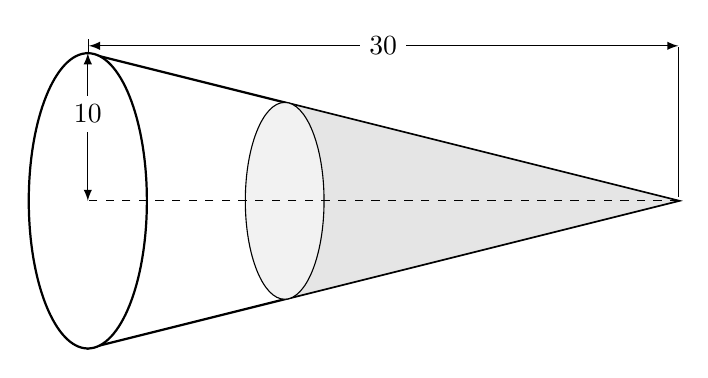
\begin{tikzpicture}[scale=0.25,yscale=0.75,important line/.style={thick}]
	\def\Hgt{30} \def\Wdt{10}	
	\def\hgt{20} \def\wdt{(\Wdt/\Hgt*\hgt}	
	\def\elw{2cm} \def\Elw{3cm}
	
	\begin{scope}[rotate=90]
		\draw [opacity=1,important line] (-\Wdt,\Hgt)-- (\Wdt,\Hgt)-- (0,0)-- cycle;%big triangle 
		\draw [important line,fill=white,opacity=1] (0,\Hgt) circle (\Wdt cm and \Elw);%top of cone 
		\draw [fill=gray!20!white,opacity=1] (-\wdt,\hgt) -- (\wdt,\hgt) -- (0,0) -- cycle;%small triangle 
		\draw [fill=gray!10!white,opacity=1] (0,\hgt) circle (\wdt cm and \elw); %top of small cone 
		\draw[dashed] (0,0) -- (0,\Hgt); %dashed lines 
		\draw[<->,>=latex] (0,\Hgt)--(\Wdt,\Hgt) node[pos=.5, above, yshift=-2pt,fill=white] {\textSize $\Wdt$};
		\draw[<->|,>=latex] (\Wdt +.5,0) -- (\Wdt +.5,\Hgt)  node[pos=.5,fill=white] {\textSize $\Hgt$}; %lenght indicator
		\draw (.25,0) -- (\Wdt +.4,0);
	\end{scope}

\end{tikzpicture}\end{center}
\end{figure}
 \renewcommand{\textSize}{\examTextSize}  \noindent The right circular
cone with a base radius of 10 centimeters and height of 30 centimeters
is to be filled with lead, as shown in the figure, and fitted as the
nose of a rocket. The shaded portion of the figure is also a right
circular cone with a height of 0.15 meters. What is the ratio of the
volume of the smaller cone to the volume of the larger cone? (The
volume of a right circular cone with base radius $r$ and height $h$
is $\frac{1}{3}\pi r^{2}h$)
\[
\frac{\,\,\,\fbox{{\ensuremath{\begin{array}{cc}
 \,  &  \answer{1} \,\end{array}}}}\,\,\,}{\fbox{{\ensuremath{\begin{array}{cc}
  &  \answer{8} \end{array}}}}}
\]
 \yspace \vfill
\item \questMulti The median and range of 117 measurements are 16 and 20,
respectively. If 11 is added to each of the 117 measurements, which
of the following statements regarding the median and range of the
modified 117 measurements must be true?

\begin{itemize}
\item The median and range will both increase.
\item The median and range will both stay the same.
\item The median will stay the same, but the range will increase.
\item The median will increase, but the range will decrease.
\item [\ansE]The median will increase, but the range will stay the same.\yspace \vfill
\end{itemize}
\item \questMulti Jill drove her mail delivery truck $10\frac{2}{3}$ miles
in $\frac{4}{5}$ of an hour. What was her average speed, in miles
per hour?

\begin{itemize}
\item $\frac{12}{115}$
\item $\frac{15}{92}$
\item $8\frac{1}{3}$
\item $8\frac{8}{15}$
\item [\ansE]$13\frac{1}{3}$\yspace \vfill
\end{itemize}
\item \questInd Determine which of the following questions are statistical
questions?\\
\\
Indiacte \textbf{all }such values.

\begin{itemize}
\item How tall is Michelle?
\item [\ansB]When do high school students eat lunch?
\item How heavy in grams is Jessica's calculus book?
\item [\ansB]How many milkshakes do customers at a ice cream chop order?\yspace \vfill
\end{itemize}
\item \questMulti Which of the following is equivalent to $-\frac{y}{5}+\frac{x}{2}$?

\begin{itemize}
\item $\frac{x-y}{2}$
\item $-\frac{x+y}{2}$
\item $5x-2y$
\item $\frac{5x-2y}{7}$
\item [\ansE]$\frac{5x-2y}{10}$\yspace \vfill
\end{itemize}
\item \questMultiPic \renewcommand{\textSize}{\examTextSize}
\begin{figure}[H]
\begin{center}%%%%%%% 
\renewcommand{\xmax}{7}
\renewcommand{\ymax}{7}
\renewcommand{\xmin}{-7}
\renewcommand{\ymin}{-7}
\begin{tikzpicture} 
\begin{axis}[
	scale=1.0,
	width=6cm,
	height=6cm,
	xmin=\xmin, xmax=\xmax,
	ymin=\ymin, ymax=\ymax,
	xtick={-6,-4,...,4,6},
	ytick={-6,-4,...,4,6},
	xticklabels={},yticklabels={},
	extra x ticks={2},extra y ticks={2},
	extra x tick style={xticklabel=\pgfmathprintnumber{\tick}},
	extra y tick style={yticklabel=\pgfmathprintnumber{\tick}},
	axis lines=middle,
	axis line style = thick,
	axis line style={-latex},
	clip=false
	] 
	\draw[very thick](axis cs:0,0) circle[radius=5.04627];
	\node[anchor=west] at (axis cs:\xmax,0) {\textSize $x$};
	\node[anchor=south] at (axis cs:0,\ymax) {\textSize $y$};
	\node[anchor=north east] at (axis cs:0,0) {\textSize $O$};

\end{axis}
\end{tikzpicture}\end{center}
\end{figure}
\renewcommand{\textSize}{\examTextSize} \noindent Which of the following
best approximates the area of the circle shown in the graph above?

\begin{itemize}
\item 16
\item 20
\item 32
\item [\ansE]80
\item 113\yspace \vfill
\end{itemize}
\item \questInd A triangle has sides of length 5, 11, and $c$. Which of
the following could be the value of $c$?\\
\\
Indicate \textbf{all }such values.

\begin{itemize}
\item $5.9$
\item [\ansB]$6.5$
\item [\ansB]$10$
\item [\ansB]$15.1$
\item $17$\yspace \vfill
\end{itemize}
\item \questMulti Jeremy planned to raise a total of $x$ investment dollars
for his startup tech business by borrowing $y$ dollars immediately
and then obtaining a fixed constant amount of dollars each week for
$w$ weeks. Which of the following expressions represents the fixed
constant amount of dollars Jeremy plans to obtain each week?

\begin{itemize}
\item $x-yw$
\item $\frac{x-w}{y}$
\item $\frac{x}{y}-w$
\item [\ansE]$\frac{x-y}{w}$
\item $\frac{x}{w}-y$\yspace \vfill
\end{itemize}
\item \questMulti If the speed of light is approximately 300,000,000 meters
per second, approximately how far does light travel in 1 minute?

\begin{itemize}
\item $3.0\times10^{8}$ meters
\item $3.0\times10^{9}$ meters
\item $1.8\times10^{9}$ meters
\item [\ansE]$1.8\times10^{10}$ meters
\item $1.8\times10^{11}$ meters\yspace \vfill
\end{itemize}
\item \questInd \renewcommand{\textSize}{\examTextSize}
\begin{figure}[H]
\begin{center}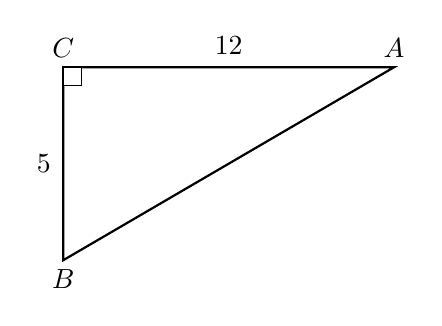
\begin{tikzpicture}[scale=.35,label style/.style={font=\textSize}]
	\coordinate (A) at (0,0); 
	\coordinate (B) at (-12,-7); 
	\coordinate (C) at (-12,0);
	\draw[thick] (A) --(B)--(C)--cycle; 
	
	\tkzMarkRightAngle[size=0.65,opacity=1,fill=white](A,C,B)
	%\tkzLabelSegment[above=1pt](A,B){ } 
	\tkzLabelSegment[left=1pt](B,C){5} 
	\tkzLabelSegment[above=1pt](C,A){12}
	%\tkzDrawPoints[color=black](A,B,C)
	\tkzLabelPoints[above](A)
	\tkzLabelPoints[below](B)     
	\tkzLabelPoints[above](C)

	%\tkzMarkAngle[size=.8cm, opacity=1.0](A,C,B) 	
	%\tkzLabelAngle[pos = 0.5](A,C,B){$65$}
		
\end{tikzpicture} \end{center}
\end{figure}
\renewcommand{\textSize}{\examTextSize} \noindent Which of the following
statements must true about the triangle $ABC$ above?\\
\\
Indicate \textbf{all }such values.

\begin{itemize}
\item The measure of angle $B$ is $45^{\circ}$.
\item [\ansB]The perimeter of the triangle is $30$.
\item The sum of the measures of angle $B$ and angle $A$ is $100$.
\item The length of side $AB$ is $17$.
\item The area of the triangle is 60.\yspace \vfill
\end{itemize}
\item \questMultiPic \renewcommand{\textSize}{\examTextSize} 
\begin{figure}[H]
\begin{center}\renewcommand{\xmax}{3.25}
\renewcommand{\xmin}{-3.25}
\renewcommand{\xstep}{0} %must be xmin+n
\renewcommand{\ymax}{5}
\renewcommand{\ymin}{0}
\renewcommand{\ystep}{0} %must be ymin+n
%%%%%%%
\begin{tikzpicture}
\begin{axis}[
	scale=1.5,
	axis lines=middle,
	axis y line=none,
	grid=none,
	xtick={-3,-2.75,-2.5,...,3},
	xticklabels={-3,,,,-2,,,,-1,,,,0,,,,1,,,,2,,,,3},
	axis line style={latex-latex}, 
	xmin=\xmin,xmax=\xmax, 
	ymin=\ymin,ymax=\ymax,
	no markers, 
	x label style={at={(axis description cs:0.5,-.25)},anchor=north},     
	y label style={at={(axis description cs:-.275,0.5)},rotate=90,anchor=south},
	clip=false, %doesn't clip outside graph
	every tick/.style={black,thick}
	]

	\addplot[only marks,mark=o,mark size=2] coordinates {(-1.75,0)} node[yshift=2pt,anchor=south]{$X$};
	\addplot[only marks,mark=o,mark size=2] coordinates {(-.75,0)} node[yshift=1pt,anchor=south]{$Y$}; %shift for q
	\addplot[only marks,mark=o,mark size=2] coordinates {(-2.5,0)} node[yshift=2pt,anchor=south]{$A$};
	\addplot[only marks,mark=o,mark size=2] coordinates {(.3,0)} node[yshift=2pt,anchor=south]{$B$};
	\addplot[only marks,mark=o,mark size=2] coordinates {(1.0,0)} node[yshift=2pt,anchor=south]{$C$};
	\addplot[only marks,mark=o,mark size=2] coordinates {(1.25,0)} node[yshift=2pt,anchor=south]{$D$};
	\addplot[only marks,mark=o,mark size=2] coordinates {(2.5,0)} node[yshift=2pt,anchor=south]{$E$};

\end{axis}
\end{tikzpicture}\end{center}
\end{figure}
\renewcommand{\textSize}{\examTextSize} \noindent The number line
above shows 7 points, each of them labeled with a letter of the alphabet.
The product of the coordinate of point $X$ and the coordinate of
point $Y$ is closest to the coordinate of which of the following
points?

\begin{itemize}
\item $A$
\item $B$
\item $C$
\item [\ansE]$D$
\item $E$\yspace \vfill\end{itemize}
\end{enumerate}

\end{document}

